
Le module de raisonnement est subdivisé en deux sous modules : le \og moteur de choix \fg{} chargé de la prise de décision et le \og moteur d'introspection \fg{} chargé d'extraire de nouvelles formes remarquables.
Le moteur de choix est chargé de la partie  prise de décision du module  de raisonnement pour ce faire celui-ci sera \og stimulé \fg{} par le module d'analyse lorsque un ensemble de plateau est disponible en mémoire. Le moteur de choix doit être capable de choisir, de façon rationnel, un plateau parmi l'ensemble proposé. Pour cela, notre IA se base sur la valuation des formes remarquables (représentées sous la forme d'une formule de logique du première ordre) associées à  nos  états de plateaux possibles. En fin de partie, elle met en œuvre un mécanisme permettant la mise à jour de la valuation des différentes \og configurations \fg{} rencontrées au cours de celle-ci en fonction du résultat final de la partie.
Le moteur d'introspection est chargé de la  partie réorganisation et évaluation des \og concepts \fg{} rencontrés. Il  examine à posteriori les raisons d'une victoire où d'une défaite grâce à  la mémoire épisodique pour optimiser ses chances de victoire futur. {+ découverte nouveaux RPBS}

Le module de raisonnement est subdivisé en deux sous modules. Le premier appelé \og moteur de choix \fg{} doit être capable de choisir, de façon rationnel, un environnement parmi un ensemble proposé. Le second appelé \og raisonneur \fg{} doit être capable de trouver de nouvelles formes remarquables à partir d'une analyse de ses diverses expériences passées.

\subsubsection{Introspection}

\paragraph{Cadre Général}

Le module d'introspection a pour objectif d'extraire, à partir des expériences passées de l'IA, de nouvelles formes remarquables potentiellement discriminante pour les choix futurs. Pour ce faire, il choisi aléatoirement, en mémoire, au moins deux environnements ayant reçu la même annotations et tente d'étendre les formes déjà connues.

\begin{figure}[H] 
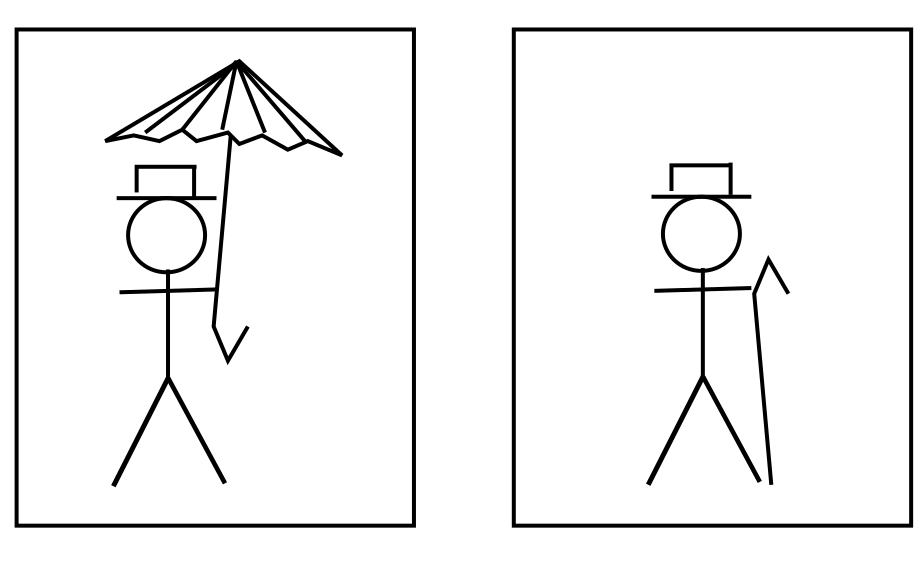
\includegraphics[width=\textwidth]{files/raisonneur/reconnaissance_de_formes_0} 
\caption{Illustration de la reconnaissance de forme} 
\label{img_reco_forme_0}
\end{figure}

Par exemple, sur la figure \ref{img_reco_forme_0}, nous considérons deux environnements présents en mémoire. Le premier représentant un homme avec un chapeau et un parapluie, le second un homme avec un chapeau et une canne. Nous souhaitons extraire de ces deux environnements la forme \og homme avec un chapeau \fg{}. Pour ce faire, ce module se base, sur les connaissances, présentent en mémoire relatives à ces environnements. En l'occurrence, nous considérerons que notre IA sait déjà reconnaître un homme et les a reconnu sur ces environnements. Notre module cherche alors à étendre, le plus possible, la forme \og homme \fg dans un des deux environnements tout en vérifiant que cette forme étendu peux toujours être injectée dans l'autre environnement, comme illustré dans la figure \ref{img_reco_forme_injection}.

\begin{figure}[H] 
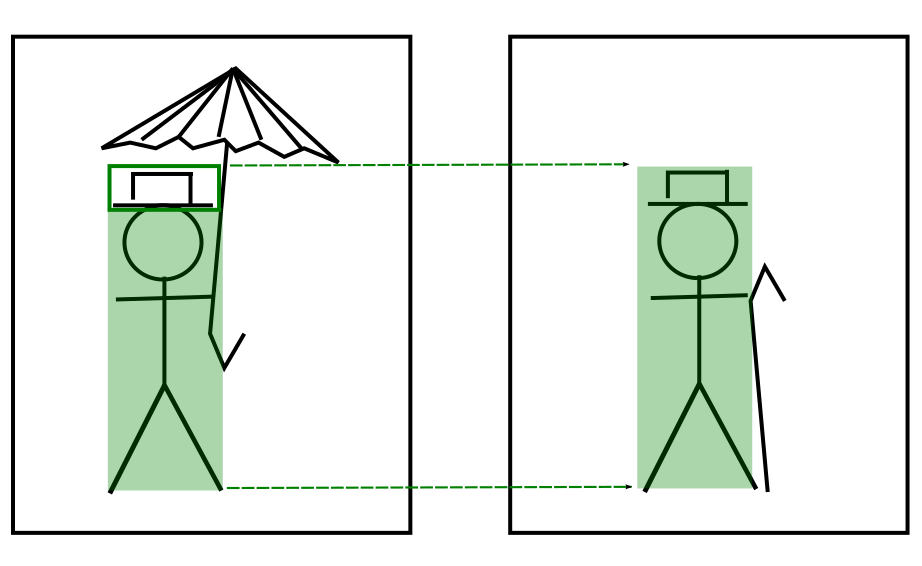
\includegraphics[width=\textwidth]{files/raisonneur/reconnaissance_de_formes_injection} 
\caption{Illustration de l'injection} 
\label{img_reco_forme_injection}
\end{figure}

\paragraph{Application aux jeux de plateau}

\begin{figure}[H] 
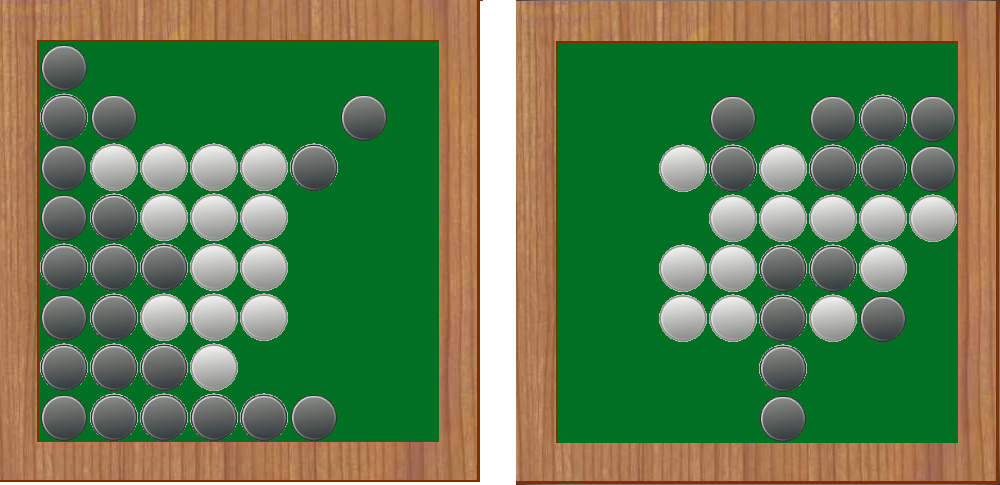
\includegraphics[width=\textwidth]{files/raisonneur/cbs_reco0} 
\caption{Illustration de l'injection} 
\label{cbs_reco0}
\end{figure}

\begin{figure}[H] 
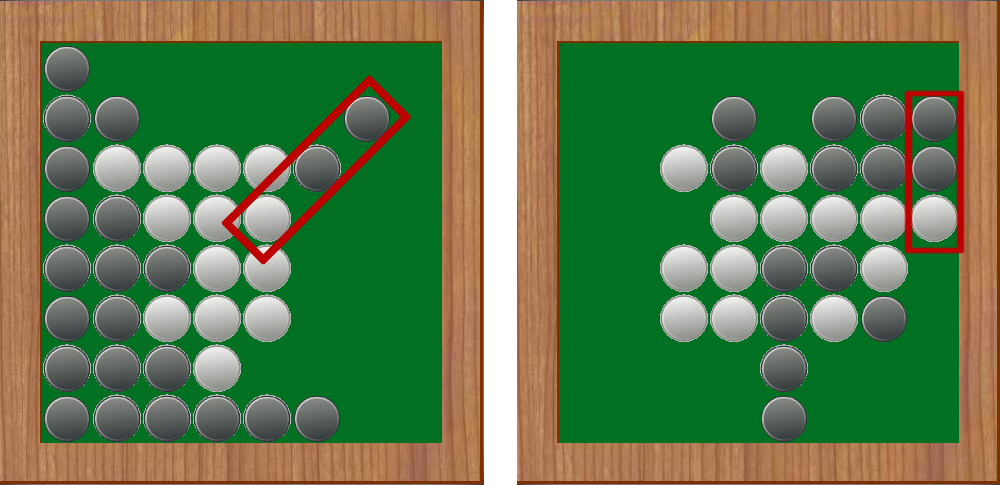
\includegraphics[width=\textwidth]{files/raisonneur/cbs_reco1} 
\caption{Illustration de l'injection} 
\label{cbs_reco1}
\end{figure}

\begin{figure}[H] 
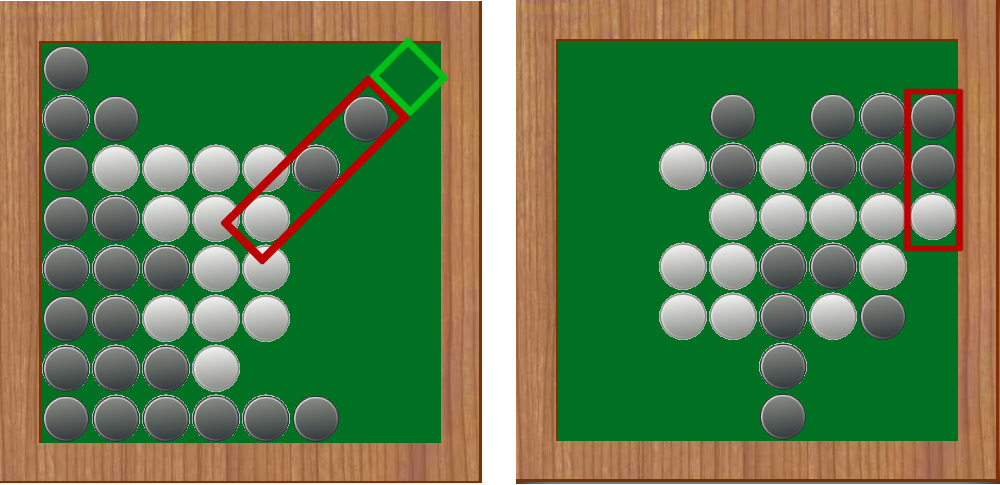
\includegraphics[width=\textwidth]{files/raisonneur/cbs_reco2} 
\caption{Illustration de l'injection} 
\label{cbs_reco2}
\end{figure}

\begin{figure}[H] 
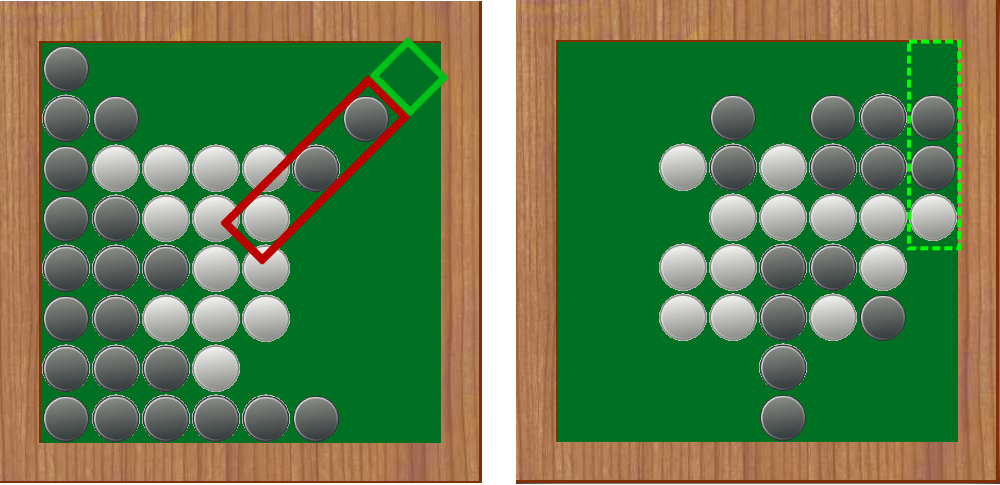
\includegraphics[width=\textwidth]{files/raisonneur/cbs_reco3} 
\caption{Illustration de l'injection} 
\label{cbs_reco3}
\end{figure}

\subsubsection{Valuation des formes}

À chaque fois que le module reçoit une annotation, celui-ci effectue une mise à jour des probabilité
\[ P(Annotation|Forme) = \frac{P(Annotation|Gain) \times P(Gain)}{P(Annotation)} \]

Par exemple, imaginons que nous souhaitons entraîner notre IA à identifier des formes géométrique basique : rond, carré, croix et triangle. Admettons que notre IA est capable de reconnaître dans son environnement les formes correspondantes mais qu'elle ne sait pas les associer au concept correspondant. Nous pouvons représenter cette état par le tableau représenté en figure \ref{img_annotations}.

\begin{figure}[H] 
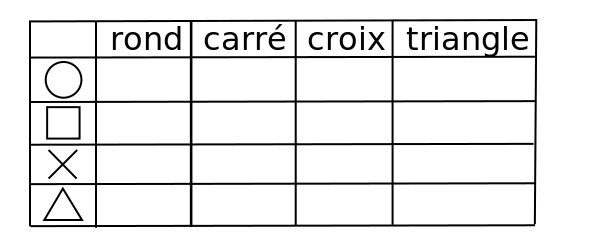
\includegraphics[width=\textwidth]{files/raisonneur/annotations} 
\caption{Association forme-concept} 
\label{img_annotations}
\end{figure}

\begin{figure}[H] 
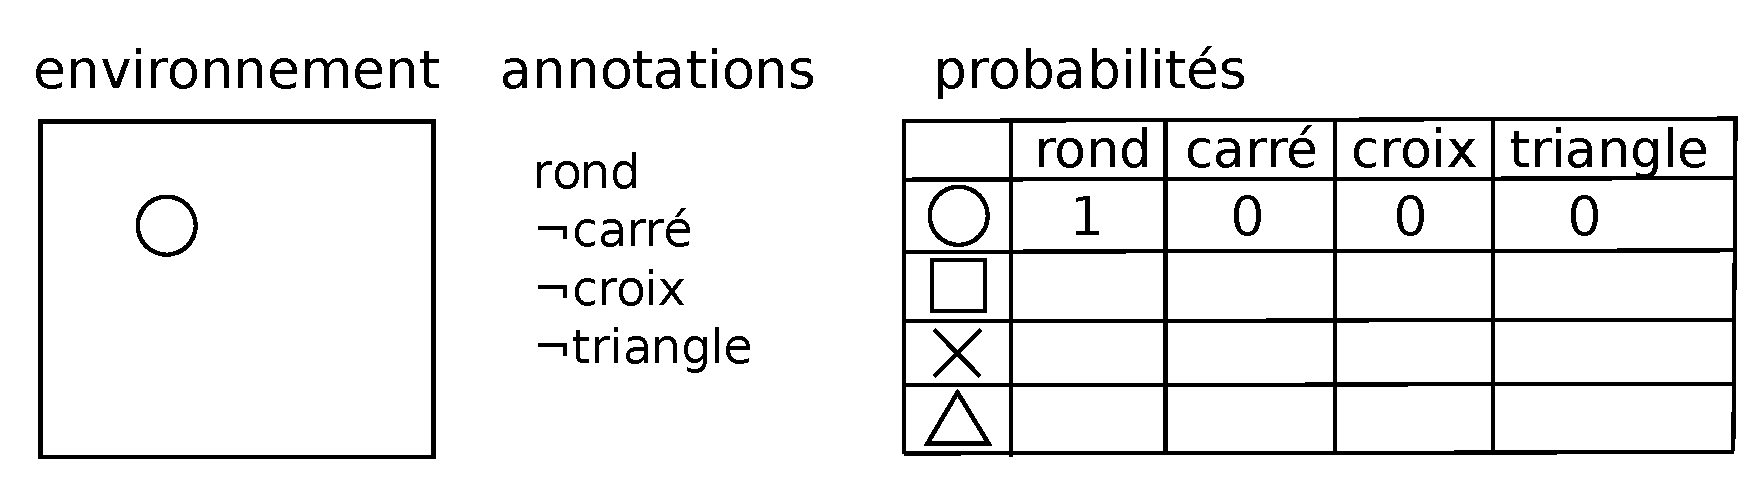
\includegraphics[width=\textwidth]{files/raisonneur/annotations_1} 
\caption{Association forme-concept 1} 
\label{img_annotations_1}
\end{figure}

\begin{figure}[H] 
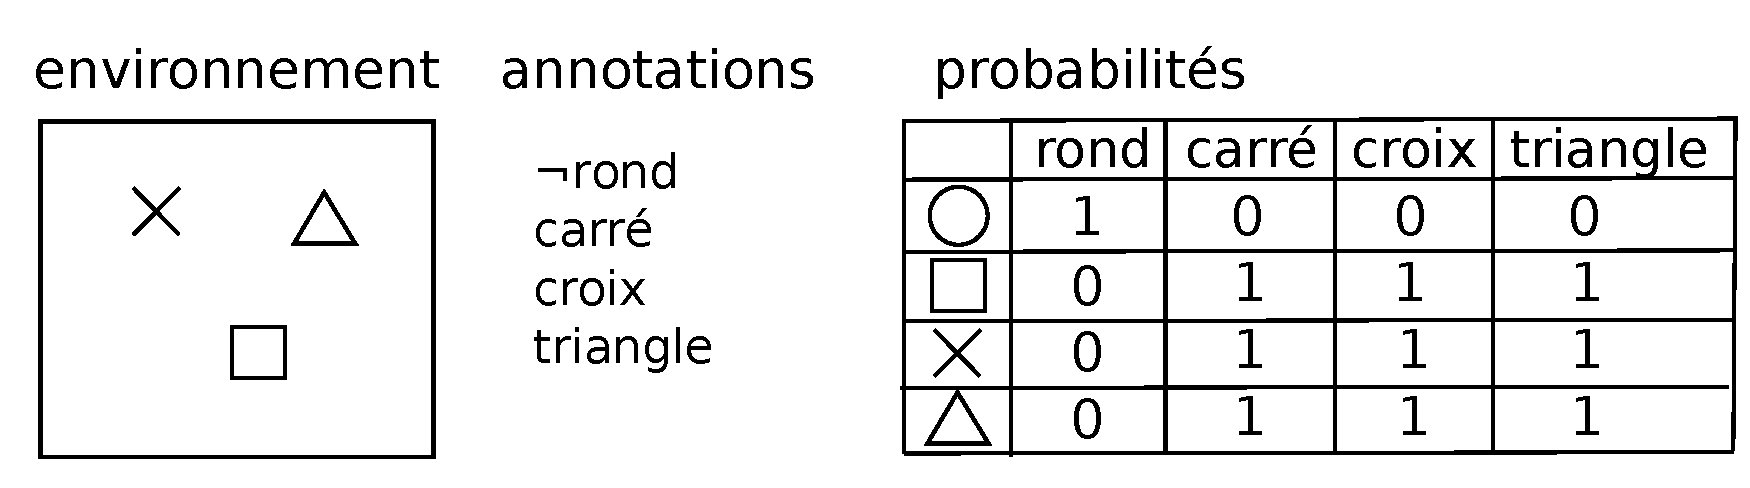
\includegraphics[width=\textwidth]{files/raisonneur/annotations_2} 
\caption{Association forme-concept 2} 
\label{img_annotations_2}
\end{figure}

\begin{figure}[H] 
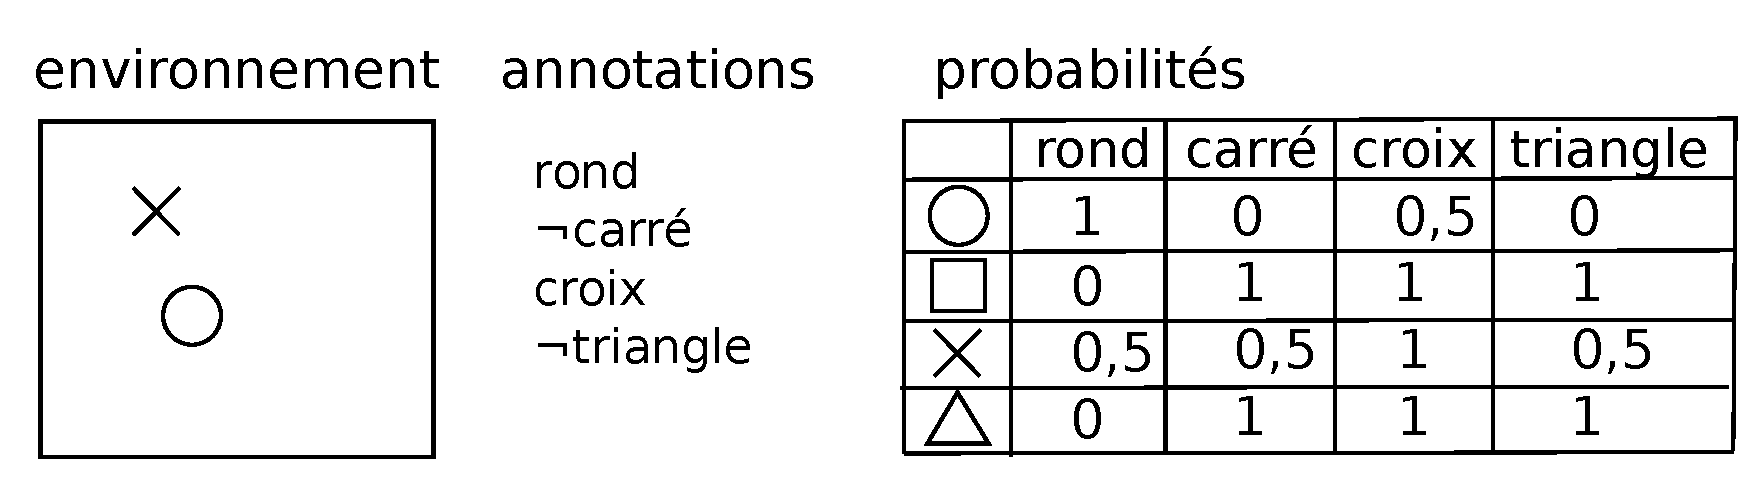
\includegraphics[width=\textwidth]{files/raisonneur/annotations_3} 
\caption{Association forme-concept 3} 
\label{img_annotations_3}
\end{figure}

\begin{figure}[H] 
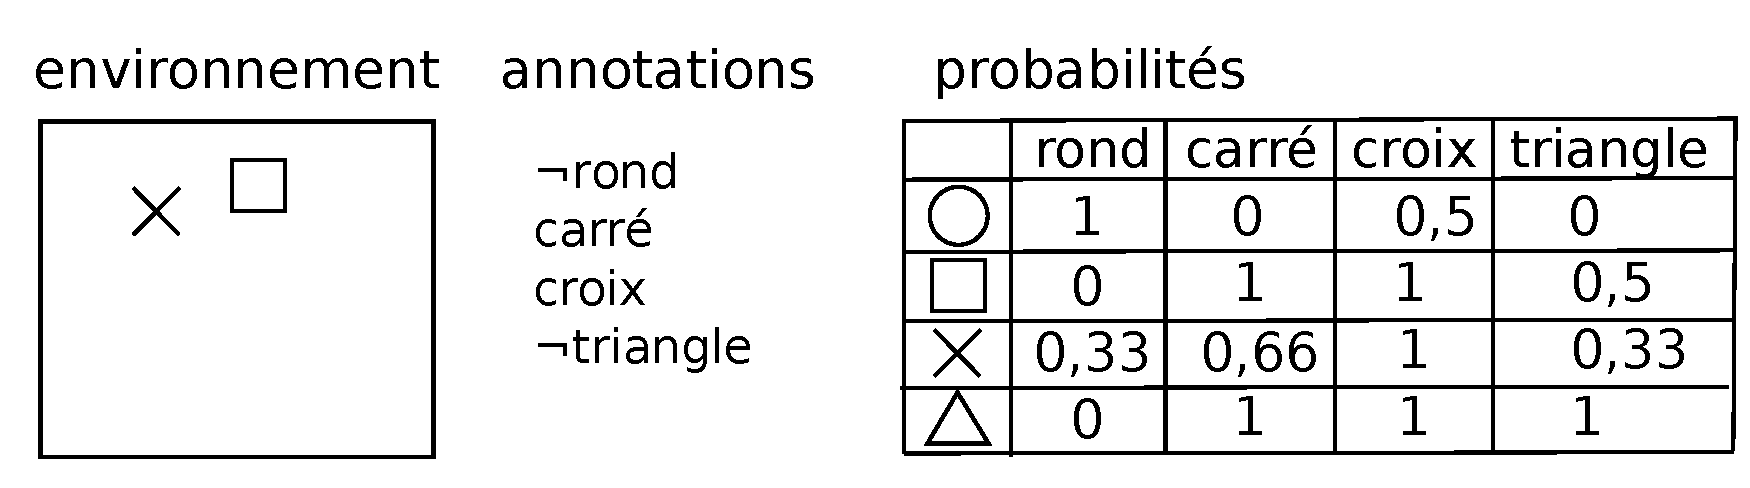
\includegraphics[width=\textwidth]{files/raisonneur/annotations_4} 
\caption{Association forme-concept 4} 
\label{img_annotations_4}
\end{figure}

\begin{figure}[H] 
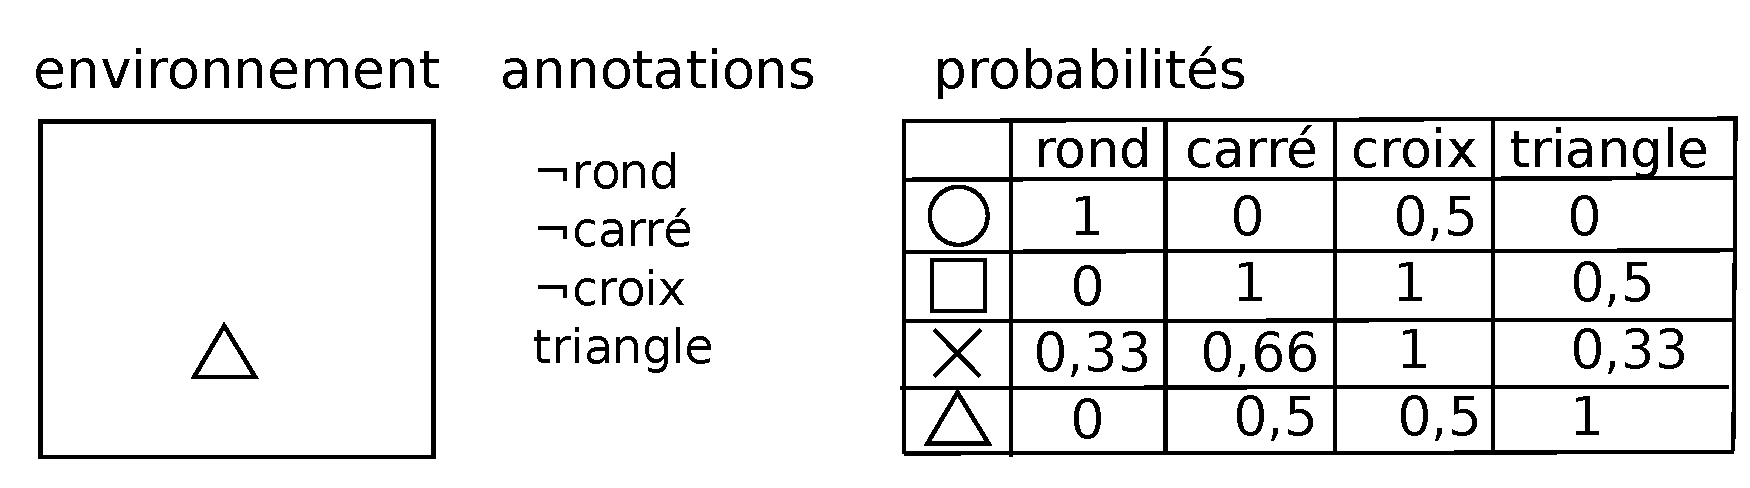
\includegraphics[width=\textwidth]{files/raisonneur/annotations_5} 
\caption{Association forme-concept 5} 
\label{img_annotations_5}
\end{figure}



\subsubsection{Moteur de choix}

\paragraph{Cadre Général}


Ce module intervient après la phase d'analyse qui lui fourni, par l'intermédiaire de la mémoire, un ensemble d'environnements possibles et pour chacun d'eux un ensemble de formes reconnues. Le \og moteur de choix \fg{} se sert alors de la probabilité d'apparition des annotations associées aux formes reconnu afin d'évaluer chaque environnement possible. Il choisi finalement l'environnement qui maximise sa fonction objectif.

\paragraph{Application aux jeux de plateau}


\begin{figure}[H] 
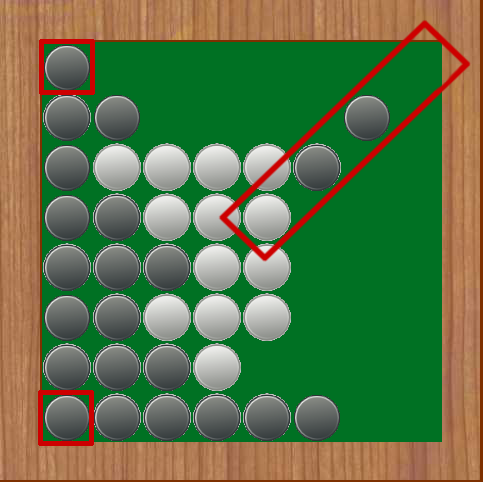
\includegraphics[width=0.3\textwidth]{files/raisonneur/moteur_de_choix} 
\caption{Représentation graphique de l'environnement} 
\label{cbs_reco0}
\end{figure}
